\documentclass[1p]{elsarticle_modified}
%\bibliographystyle{elsarticle-num}

%\usepackage[colorlinks]{hyperref}
%\usepackage{abbrmath_seonhwa} %\Abb, \Ascr, \Acal ,\Abf, \Afrak
\usepackage{amsfonts}
\usepackage{amssymb}
\usepackage{amsmath}
\usepackage{amsthm}
\usepackage{scalefnt}
\usepackage{amsbsy}
\usepackage{kotex}
\usepackage{caption}
\usepackage{subfig}
\usepackage{color}
\usepackage{graphicx}
\usepackage{xcolor} %% white, black, red, green, blue, cyan, magenta, yellow
\usepackage{float}
\usepackage{setspace}
\usepackage{hyperref}

\usepackage{tikz}
\usetikzlibrary{arrows}

\usepackage{multirow}
\usepackage{array} % fixed length table
\usepackage{hhline}

%%%%%%%%%%%%%%%%%%%%%
\makeatletter
\renewcommand*\env@matrix[1][\arraystretch]{%
	\edef\arraystretch{#1}%
	\hskip -\arraycolsep
	\let\@ifnextchar\new@ifnextchar
	\array{*\c@MaxMatrixCols c}}
\makeatother %https://tex.stackexchange.com/questions/14071/how-can-i-increase-the-line-spacing-in-a-matrix
%%%%%%%%%%%%%%%

\usepackage[normalem]{ulem}

\newcommand{\msout}[1]{\ifmmode\text{\sout{\ensuremath{#1}}}\else\sout{#1}\fi}
%SOURCE: \msout is \stkout macro in https://tex.stackexchange.com/questions/20609/strikeout-in-math-mode

\newcommand{\cancel}[1]{
	\ifmmode
	{\color{red}\msout{#1}}
	\else
	{\color{red}\sout{#1}}
	\fi
}

\newcommand{\add}[1]{
	{\color{blue}\uwave{#1}}
}

\newcommand{\replace}[2]{
	\ifmmode
	{\color{red}\msout{#1}}{\color{blue}\uwave{#2}}
	\else
	{\color{red}\sout{#1}}{\color{blue}\uwave{#2}}
	\fi
}

\newcommand{\Sol}{\mathcal{S}} %segment
\newcommand{\D}{D} %diagram
\newcommand{\A}{\mathcal{A}} %arc


%%%%%%%%%%%%%%%%%%%%%%%%%%%%%5 test

\def\sl{\operatorname{\textup{SL}}(2,\Cbb)}
\def\psl{\operatorname{\textup{PSL}}(2,\Cbb)}
\def\quan{\mkern 1mu \triangleright \mkern 1mu}

\theoremstyle{definition}
\newtheorem{thm}{Theorem}[section]
\newtheorem{prop}[thm]{Proposition}
\newtheorem{lem}[thm]{Lemma}
\newtheorem{ques}[thm]{Question}
\newtheorem{cor}[thm]{Corollary}
\newtheorem{defn}[thm]{Definition}
\newtheorem{exam}[thm]{Example}
\newtheorem{rmk}[thm]{Remark}
\newtheorem{alg}[thm]{Algorithm}

\newcommand{\I}{\sqrt{-1}}
\begin{document}

%\begin{frontmatter}
%
%\title{Boundary parabolic representations of knots up to 8 crossings}
%
%%% Group authors per affiliation:
%\author{Yunhi Cho} 
%\address{Department of Mathematics, University of Seoul, Seoul, Korea}
%\ead{yhcho@uos.ac.kr}
%
%
%\author{Seonhwa Kim} %\fnref{s_kim}}
%\address{Center for Geometry and Physics, Institute for Basic Science, Pohang, 37673, Korea}
%\ead{ryeona17@ibs.re.kr}
%
%\author{Hyuk Kim}
%\address{Department of Mathematical Sciences, Seoul National University, Seoul 08826, Korea}
%\ead{hyukkim@snu.ac.kr}
%
%\author{Seokbeom Yoon}
%\address{Department of Mathematical Sciences, Seoul National University, Seoul, 08826,  Korea}
%\ead{sbyoon15@snu.ac.kr}
%
%\begin{abstract}
%We find all boundary parabolic representation of knots up to 8 crossings.
%
%\end{abstract}
%\begin{keyword}
%    \MSC[2010] 57M25 
%\end{keyword}
%
%\end{frontmatter}

%\linenumbers
%\tableofcontents
%
\newcommand\colored[1]{\textcolor{white}{\rule[-0.35ex]{0.8em}{1.4ex}}\kern-0.8em\color{red} #1}%
%\newcommand\colored[1]{\textcolor{white}{ #1}\kern-2.17ex	\textcolor{white}{ #1}\kern-1.81ex	\textcolor{white}{ #1}\kern-2.15ex\color{red}#1	}

{\Large $\underline{12a_{1045}~(K12a_{1045})}$}

\setlength{\tabcolsep}{10pt}
\renewcommand{\arraystretch}{1.6}
\vspace{1cm}\begin{tabular}{m{100pt}>{\centering\arraybackslash}m{274pt}}
\multirow{5}{120pt}{
	\centering
	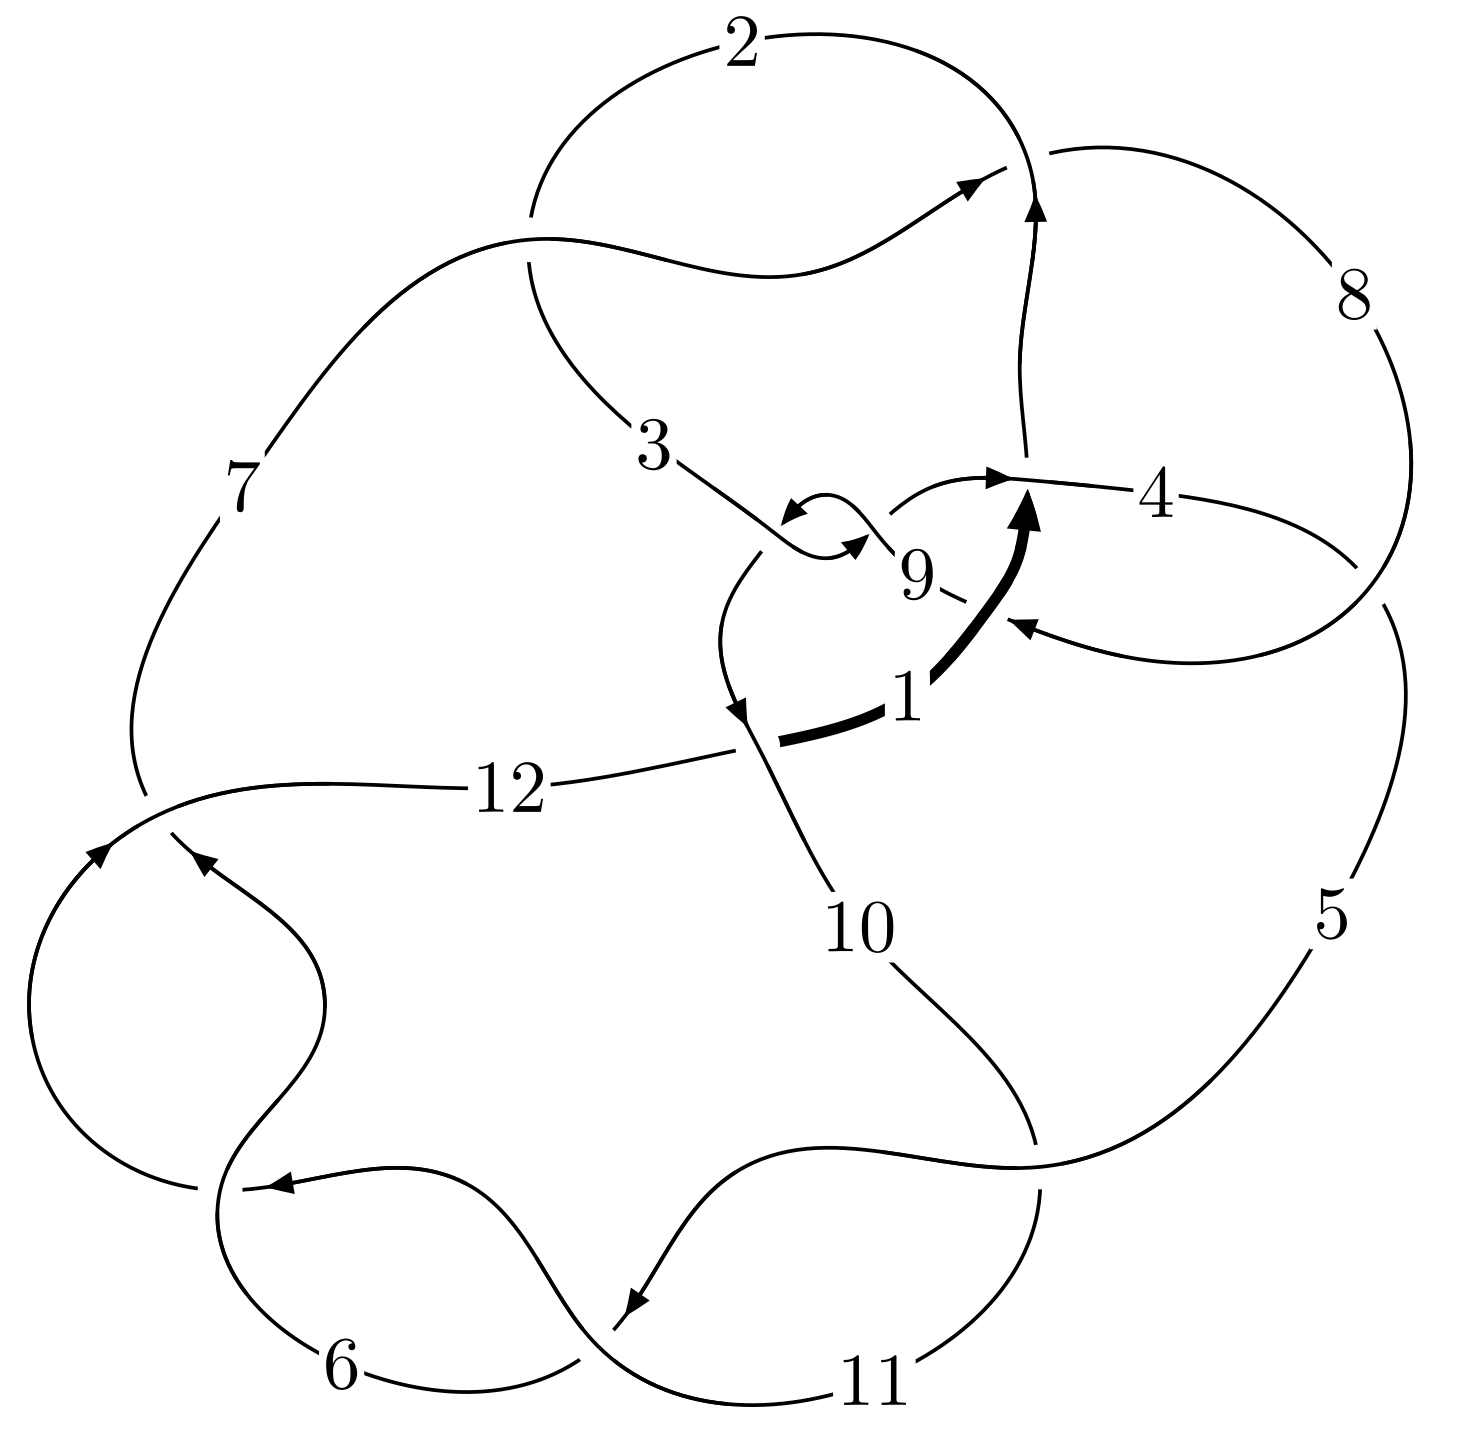
\includegraphics[width=112pt]{../../../GIT/diagram.site/Diagrams/png/1846_12a_1045.png}\\
\ \ \ A knot diagram\footnotemark}&
\allowdisplaybreaks
\textbf{Linearized knot diagam} \\
\cline{2-2}
 &
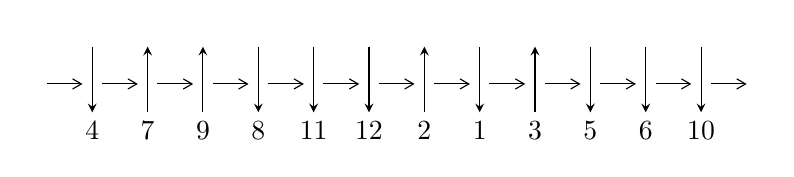
\begin{tikzpicture}[x=20pt, y=17pt]
	% nodes
	\node (C0) at (0, 0) {};
	\node (C1) at (1, 0) {};
	\node (C1U) at (1, +1) {};
	\node (C1D) at (1, -1) {4};

	\node (C2) at (2, 0) {};
	\node (C2U) at (2, +1) {};
	\node (C2D) at (2, -1) {7};

	\node (C3) at (3, 0) {};
	\node (C3U) at (3, +1) {};
	\node (C3D) at (3, -1) {9};

	\node (C4) at (4, 0) {};
	\node (C4U) at (4, +1) {};
	\node (C4D) at (4, -1) {8};

	\node (C5) at (5, 0) {};
	\node (C5U) at (5, +1) {};
	\node (C5D) at (5, -1) {11};

	\node (C6) at (6, 0) {};
	\node (C6U) at (6, +1) {};
	\node (C6D) at (6, -1) {12};

	\node (C7) at (7, 0) {};
	\node (C7U) at (7, +1) {};
	\node (C7D) at (7, -1) {2};

	\node (C8) at (8, 0) {};
	\node (C8U) at (8, +1) {};
	\node (C8D) at (8, -1) {1};

	\node (C9) at (9, 0) {};
	\node (C9U) at (9, +1) {};
	\node (C9D) at (9, -1) {3};

	\node (C10) at (10, 0) {};
	\node (C10U) at (10, +1) {};
	\node (C10D) at (10, -1) {5};

	\node (C11) at (11, 0) {};
	\node (C11U) at (11, +1) {};
	\node (C11D) at (11, -1) {6};

	\node (C12) at (12, 0) {};
	\node (C12U) at (12, +1) {};
	\node (C12D) at (12, -1) {10};
	\node (C13) at (13, 0) {};

	% arrows
	\draw[->,>={angle 60}]
	(C0) edge (C1) (C1) edge (C2) (C2) edge (C3) (C3) edge (C4) (C4) edge (C5) (C5) edge (C6) (C6) edge (C7) (C7) edge (C8) (C8) edge (C9) (C9) edge (C10) (C10) edge (C11) (C11) edge (C12) (C12) edge (C13) ;	\draw[->,>=stealth]
	(C1U) edge (C1D) (C2D) edge (C2U) (C3D) edge (C3U) (C4U) edge (C4D) (C5U) edge (C5D) (C6U) edge (C6D) (C7D) edge (C7U) (C8U) edge (C8D) (C9D) edge (C9U) (C10U) edge (C10D) (C11U) edge (C11D) (C12U) edge (C12D) ;
	\end{tikzpicture} \\
\hhline{~~} \\& 
\textbf{Solving Sequence} \\ \cline{2-2} 
 &
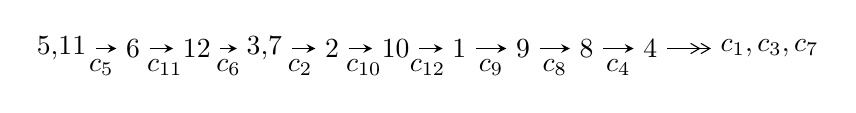
\begin{tikzpicture}[x=23pt, y=7pt]
	% node
	\node (A0) at (-1/8, 0) {5,11};
	\node (A1) at (1, 0) {6};
	\node (A2) at (2, 0) {12};
	\node (A3) at (49/16, 0) {3,7};
	\node (A4) at (33/8, 0) {2};
	\node (A5) at (41/8, 0) {10};
	\node (A6) at (49/8, 0) {1};
	\node (A7) at (57/8, 0) {9};
	\node (A8) at (65/8, 0) {8};
	\node (A9) at (73/8, 0) {4};
	\node (C1) at (1/2, -1) {$c_{5}$};
	\node (C2) at (3/2, -1) {$c_{11}$};
	\node (C3) at (5/2, -1) {$c_{6}$};
	\node (C4) at (29/8, -1) {$c_{2}$};
	\node (C5) at (37/8, -1) {$c_{10}$};
	\node (C6) at (45/8, -1) {$c_{12}$};
	\node (C7) at (53/8, -1) {$c_{9}$};
	\node (C8) at (61/8, -1) {$c_{8}$};
	\node (C9) at (69/8, -1) {$c_{4}$};
	\node (A10) at (11, 0) {$c_{1},c_{3},c_{7}$};

	% edge
	\draw[->,>=stealth]	
	(A0) edge (A1) (A1) edge (A2) (A2) edge (A3) (A3) edge (A4) (A4) edge (A5) (A5) edge (A6) (A6) edge (A7) (A7) edge (A8) (A8) edge (A9) ;
	\draw[->>,>={angle 60}]	
	(A9) edge (A10);
\end{tikzpicture} \\ 

\end{tabular} \\

\footnotetext{
The image of knot diagram is generated by the software ``\textbf{Draw programme}" developed by Andrew Bartholomew(\url{http://www.layer8.co.uk/maths/draw/index.htm\#Running-draw}), where we modified some parts for our purpose(\url{https://github.com/CATsTAILs/LinksPainter}).
}\phantom \\ \newline 
\centering \textbf{Ideals for irreducible components\footnotemark of $X_{\text{par}}$} 
 
\begin{align*}
I^u_{1}&=\langle 
-233 u^{29}+1283 u^{28}+\cdots+4 b-1220,\;-533 u^{29}+2893 u^{28}+\cdots+8 a-2692,\\
\phantom{I^u_{1}}&\phantom{= \langle  }u^{30}-7 u^{29}+\cdots-4 u-8\rangle \\
I^u_{2}&=\langle 
4.20118\times10^{22} a^{5} u^{10}+5.48121\times10^{23} a^{4} u^{10}+\cdots+3.93261\times10^{24} a-4.34401\times10^{24},\\
\phantom{I^u_{2}}&\phantom{= \langle  }u^{10} a^5+5 u^{10} a^4+\cdots+5 a-3,\;u^{11}+u^{10}-6 u^9-5 u^8+12 u^7+6 u^6-10 u^5+u^4+5 u^3- u^2+1\rangle \\
I^u_{3}&=\langle 
- u^{14}+2 u^{13}+8 u^{12}-15 u^{11}-24 u^{10}+39 u^9+36 u^8-38 u^7-37 u^6+8 u^5+32 u^4-12 u^2+b-2 u+2,\\
\phantom{I^u_{3}}&\phantom{= \langle  }-2 u^{14}+2 u^{13}+\cdots+a+2,\\
\phantom{I^u_{3}}&\phantom{= \langle  }u^{16}-10 u^{14}+39 u^{12}+u^{11}-74 u^{10}-8 u^9+71 u^8+23 u^7-38 u^6-28 u^5+18 u^4+13 u^3-4 u^2-2 u+1\rangle \\
\\
\end{align*}
\raggedright * 3 irreducible components of $\dim_{\mathbb{C}}=0$, with total 112 representations.\\
\footnotetext{All coefficients of polynomials are rational numbers. But the coefficients are sometimes approximated in decimal forms when there is not enough margin.}
\newpage
\renewcommand{\arraystretch}{1}
\centering \section*{I. $I^u_{1}= \langle -233 u^{29}+1283 u^{28}+\cdots+4 b-1220,\;-533 u^{29}+2893 u^{28}+\cdots+8 a-2692,\;u^{30}-7 u^{29}+\cdots-4 u-8 \rangle$}
\flushleft \textbf{(i) Arc colorings}\\
\begin{tabular}{m{7pt} m{180pt} m{7pt} m{180pt} }
\flushright $a_{5}=$&$\begin{pmatrix}1\\0\end{pmatrix}$ \\
\flushright $a_{11}=$&$\begin{pmatrix}0\\u\end{pmatrix}$ \\
\flushright $a_{6}=$&$\begin{pmatrix}1\\u^2\end{pmatrix}$ \\
\flushright $a_{12}=$&$\begin{pmatrix}- u\\- u^3+u\end{pmatrix}$ \\
\flushright $a_{3}=$&$\begin{pmatrix}66.6250 u^{29}-361.625 u^{28}+\cdots+373.250 u+336.500\\\frac{233}{4} u^{29}-\frac{1283}{4} u^{28}+\cdots+349 u+305\end{pmatrix}$ \\
\flushright $a_{7}=$&$\begin{pmatrix}- u^2+1\\- u^4+2 u^2\end{pmatrix}$ \\
\flushright $a_{2}=$&$\begin{pmatrix}22.3750 u^{29}-127.875 u^{28}+\cdots+160.250 u+131.500\\-\frac{31}{4} u^{29}+\frac{157}{4} u^{28}+\cdots-31 u-31\end{pmatrix}$ \\
\flushright $a_{10}=$&$\begin{pmatrix}u\\u\end{pmatrix}$ \\
\flushright $a_{1}=$&$\begin{pmatrix}u^5-2 u^3- u\\u^5-3 u^3+u\end{pmatrix}$ \\
\flushright $a_{9}=$&$\begin{pmatrix}\frac{41}{8} u^{29}-\frac{289}{8} u^{28}+\cdots+\frac{329}{4} u+56\\-\frac{53}{4} u^{29}+\frac{261}{4} u^{28}+\cdots-\frac{71}{2} u-43\end{pmatrix}$ \\
\flushright $a_{8}=$&$\begin{pmatrix}\frac{197}{8} u^{29}-\frac{1045}{8} u^{28}+\cdots+\frac{489}{4} u+114\\\frac{49}{4} u^{29}-\frac{265}{4} u^{28}+\cdots+\frac{129}{2} u+59\end{pmatrix}$ \\
\flushright $a_{4}=$&$\begin{pmatrix}\frac{109}{8} u^{29}-\frac{571}{8} u^{28}+\cdots+65 u+64\\\frac{63}{2} u^{29}-173 u^{28}+\cdots+\frac{381}{2} u+165\end{pmatrix}$\\&\end{tabular}
\flushleft \textbf{(ii) Obstruction class $= -1$}\\~\\
\flushleft \textbf{(iii) Cusp Shapes $= -43 u^{29}+233 u^{28}+24 u^{27}-2066 u^{26}+1935 u^{25}+7589 u^{24}-8992 u^{23}-18142 u^{22}+17380 u^{21}+37598 u^{20}-16730 u^{19}-60970 u^{18}-3411 u^{17}+65829 u^{16}+39349 u^{15}-41950 u^{14}-51488 u^{13}-4016 u^{12}+34851 u^{11}+20846 u^{10}-921 u^9-13945 u^8-6633 u^7-1648 u^6+2861 u^5+1809 u^4+1337 u^3-166 u^2-248 u-210$}\\~\\
\newpage\renewcommand{\arraystretch}{1}
\flushleft \textbf{(iv) u-Polynomials at the component}\newline \\
\begin{tabular}{m{50pt}|m{274pt}}
Crossings & \hspace{64pt}u-Polynomials at each crossing \\
\hline $$\begin{aligned}c_{1}\end{aligned}$$&$\begin{aligned}
&u^{30}-27 u^{29}+\cdots-36864 u+2048
\end{aligned}$\\
\hline $$\begin{aligned}c_{2},c_{3},c_{7}\\c_{9}\end{aligned}$$&$\begin{aligned}
&u^{30}+11 u^{28}+\cdots+u-1
\end{aligned}$\\
\hline $$\begin{aligned}c_{4},c_{8}\end{aligned}$$&$\begin{aligned}
&u^{30}+u^{29}+\cdots-2 u-1
\end{aligned}$\\
\hline $$\begin{aligned}c_{5},c_{6},c_{10}\\c_{11}\end{aligned}$$&$\begin{aligned}
&u^{30}+7 u^{29}+\cdots+4 u-8
\end{aligned}$\\
\hline $$\begin{aligned}c_{12}\end{aligned}$$&$\begin{aligned}
&u^{30}-7 u^{29}+\cdots+56384 u-20992
\end{aligned}$\\
\hline
\end{tabular}\\~\\
\newpage\renewcommand{\arraystretch}{1}
\flushleft \textbf{(v) Riley Polynomials at the component}\newline \\
\begin{tabular}{m{50pt}|m{274pt}}
Crossings & \hspace{64pt}Riley Polynomials at each crossing \\
\hline $$\begin{aligned}c_{1}\end{aligned}$$&$\begin{aligned}
&y^{30}-9 y^{29}+\cdots-48234496 y+4194304
\end{aligned}$\\
\hline $$\begin{aligned}c_{2},c_{3},c_{7}\\c_{9}\end{aligned}$$&$\begin{aligned}
&y^{30}+22 y^{29}+\cdots-11 y+1
\end{aligned}$\\
\hline $$\begin{aligned}c_{4},c_{8}\end{aligned}$$&$\begin{aligned}
&y^{30}+3 y^{29}+\cdots+12 y+1
\end{aligned}$\\
\hline $$\begin{aligned}c_{5},c_{6},c_{10}\\c_{11}\end{aligned}$$&$\begin{aligned}
&y^{30}-33 y^{29}+\cdots-16 y+64
\end{aligned}$\\
\hline $$\begin{aligned}c_{12}\end{aligned}$$&$\begin{aligned}
&y^{30}+3 y^{29}+\cdots-206688256 y+440664064
\end{aligned}$\\
\hline
\end{tabular}\\~\\
\newpage\flushleft \textbf{(vi) Complex Volumes and Cusp Shapes}
$$\begin{array}{c|c|c}  
\text{Solutions to }I^u_{1}& \I (\text{vol} + \sqrt{-1}CS) & \text{Cusp shape}\\
 \hline 
\begin{aligned}
u &= -0.863405 + 0.530291 I \\
a &= -0.684999 + 0.008143 I \\
b &= -0.897675 + 1.001320 I\end{aligned}
 & -3.01285 + 5.42239 I & -5.0249 - 13.7215 I \\ \hline\begin{aligned}
u &= -0.863405 - 0.530291 I \\
a &= -0.684999 - 0.008143 I \\
b &= -0.897675 - 1.001320 I\end{aligned}
 & -3.01285 - 5.42239 I & -5.0249 + 13.7215 I \\ \hline\begin{aligned}
u &= -0.731476 + 0.568139 I \\
a &= \phantom{-}1.114310 + 0.365338 I \\
b &= \phantom{-}1.56285 - 1.21446 I\end{aligned}
 & -6.0916 + 13.9505 I & -9.16482 - 9.63284 I \\ \hline\begin{aligned}
u &= -0.731476 - 0.568139 I \\
a &= \phantom{-}1.114310 - 0.365338 I \\
b &= \phantom{-}1.56285 + 1.21446 I\end{aligned}
 & -6.0916 - 13.9505 I & -9.16482 + 9.63284 I \\ \hline\begin{aligned}
u &= \phantom{-}1.051940 + 0.292196 I \\
a &= -0.289301 - 1.130000 I \\
b &= \phantom{-}0.373374 - 0.058569 I\end{aligned}
 & -8.43524 + 6.26787 I & -11.74379 - 3.92525 I \\ \hline\begin{aligned}
u &= \phantom{-}1.051940 - 0.292196 I \\
a &= -0.289301 + 1.130000 I \\
b &= \phantom{-}0.373374 + 0.058569 I\end{aligned}
 & -8.43524 - 6.26787 I & -11.74379 + 3.92525 I \\ \hline\begin{aligned}
u &= -0.484434 + 0.766175 I \\
a &= -0.062606 - 0.648073 I \\
b &= -0.985885 + 0.008839 I\end{aligned}
 & -1.10337 + 2.52152 I & -5.89538 - 5.05949 I \\ \hline\begin{aligned}
u &= -0.484434 - 0.766175 I \\
a &= -0.062606 + 0.648073 I \\
b &= -0.985885 - 0.008839 I\end{aligned}
 & -1.10337 - 2.52152 I & -5.89538 + 5.05949 I \\ \hline\begin{aligned}
u &= -0.548147 + 0.512523 I \\
a &= -0.706260 + 0.439855 I \\
b &= \phantom{-}0.058759 + 1.016530 I\end{aligned}
 & \phantom{-}2.18720 + 3.47846 I & -0.09259 - 5.90060 I \\ \hline\begin{aligned}
u &= -0.548147 - 0.512523 I \\
a &= -0.706260 - 0.439855 I \\
b &= \phantom{-}0.058759 - 1.016530 I\end{aligned}
 & \phantom{-}2.18720 - 3.47846 I & -0.09259 + 5.90060 I\\
 \hline 
 \end{array}$$\newpage$$\begin{array}{c|c|c}  
\text{Solutions to }I^u_{1}& \I (\text{vol} + \sqrt{-1}CS) & \text{Cusp shape}\\
 \hline 
\begin{aligned}
u &= -0.192741 + 0.695844 I \\
a &= -1.071720 + 0.672690 I \\
b &= \phantom{-}0.921075 + 0.862157 I\end{aligned}
 & -4.48729 - 9.71321 I & -6.59814 + 5.23923 I \\ \hline\begin{aligned}
u &= -0.192741 - 0.695844 I \\
a &= -1.071720 - 0.672690 I \\
b &= \phantom{-}0.921075 - 0.862157 I\end{aligned}
 & -4.48729 + 9.71321 I & -6.59814 - 5.23923 I \\ \hline\begin{aligned}
u &= -0.388423 + 0.514575 I \\
a &= \phantom{-}0.941435 + 0.297487 I \\
b &= \phantom{-}0.530431 - 0.779112 I\end{aligned}
 & \phantom{-}2.64855 + 0.09639 I & \phantom{-}1.44482 - 2.17887 I \\ \hline\begin{aligned}
u &= -0.388423 - 0.514575 I \\
a &= \phantom{-}0.941435 - 0.297487 I \\
b &= \phantom{-}0.530431 + 0.779112 I\end{aligned}
 & \phantom{-}2.64855 - 0.09639 I & \phantom{-}1.44482 + 2.17887 I \\ \hline\begin{aligned}
u &= \phantom{-}0.106548 + 0.589026 I \\
a &= \phantom{-}0.822013 + 0.171417 I \\
b &= -0.283998 - 0.456801 I\end{aligned}
 & -0.17771 - 1.54871 I & -0.18007 + 2.74695 I \\ \hline\begin{aligned}
u &= \phantom{-}0.106548 - 0.589026 I \\
a &= \phantom{-}0.822013 - 0.171417 I \\
b &= -0.283998 + 0.456801 I\end{aligned}
 & -0.17771 + 1.54871 I & -0.18007 - 2.74695 I \\ \hline\begin{aligned}
u &= \phantom{-}0.596209\phantom{ +0.000000I} \\
a &= \phantom{-}0.544746\phantom{ +0.000000I} \\
b &= -0.131144\phantom{ +0.000000I}\end{aligned}
 & -1.09004\phantom{ +0.000000I} & -8.37530\phantom{ +0.000000I} \\ \hline\begin{aligned}
u &= \phantom{-}1.41655 + 0.25699 I \\
a &= -0.808360 + 0.799987 I \\
b &= -0.800464 + 0.038413 I\end{aligned}
 & -7.16962 - 6.25363 I & -10.89356 + 7.51977 I \\ \hline\begin{aligned}
u &= \phantom{-}1.41655 - 0.25699 I \\
a &= -0.808360 - 0.799987 I \\
b &= -0.800464 - 0.038413 I\end{aligned}
 & -7.16962 + 6.25363 I & -10.89356 - 7.51977 I \\ \hline\begin{aligned}
u &= \phantom{-}1.48803 + 0.08948 I \\
a &= \phantom{-}1.73464 + 0.05380 I \\
b &= \phantom{-}1.236300 + 0.345342 I\end{aligned}
 & -3.44648 - 2.04173 I & \phantom{-0.000000 } 0\\
 \hline 
 \end{array}$$\newpage$$\begin{array}{c|c|c}  
\text{Solutions to }I^u_{1}& \I (\text{vol} + \sqrt{-1}CS) & \text{Cusp shape}\\
 \hline 
\begin{aligned}
u &= \phantom{-}1.48803 - 0.08948 I \\
a &= \phantom{-}1.73464 - 0.05380 I \\
b &= \phantom{-}1.236300 - 0.345342 I\end{aligned}
 & -3.44648 + 2.04173 I & \phantom{-0.000000 } 0 \\ \hline\begin{aligned}
u &= \phantom{-}1.54359 + 0.14330 I \\
a &= -0.818557 - 1.014570 I \\
b &= -0.366568 - 1.075300 I\end{aligned}
 & -4.79663 - 5.82343 I & \phantom{-0.000000 } 0 \\ \hline\begin{aligned}
u &= \phantom{-}1.54359 - 0.14330 I \\
a &= -0.818557 + 1.014570 I \\
b &= -0.366568 + 1.075300 I\end{aligned}
 & -4.79663 + 5.82343 I & \phantom{-0.000000 } 0 \\ \hline\begin{aligned}
u &= -1.55904\phantom{ +0.000000I} \\
a &= -0.0976328\phantom{ +0.000000I} \\
b &= -0.389520\phantom{ +0.000000I}\end{aligned}
 & -8.42781\phantom{ +0.000000I} & -9.45490\phantom{ +0.000000I} \\ \hline\begin{aligned}
u &= \phantom{-}1.61572 + 0.17130 I \\
a &= \phantom{-}2.49295 + 0.48824 I \\
b &= \phantom{-}2.22027 + 1.42432 I\end{aligned}
 & -14.0241 - 16.7372 I & \phantom{-0.000000 } 0 \\ \hline\begin{aligned}
u &= \phantom{-}1.61572 - 0.17130 I \\
a &= \phantom{-}2.49295 - 0.48824 I \\
b &= \phantom{-}2.22027 - 1.42432 I\end{aligned}
 & -14.0241 + 16.7372 I & \phantom{-0.000000 } 0 \\ \hline\begin{aligned}
u &= \phantom{-}1.65106 + 0.16927 I \\
a &= -1.69282 - 0.62506 I \\
b &= -1.52761 - 1.31367 I\end{aligned}
 & -11.5587 - 8.1943 I & \phantom{-0.000000 } 0 \\ \hline\begin{aligned}
u &= \phantom{-}1.65106 - 0.16927 I \\
a &= -1.69282 + 0.62506 I \\
b &= -1.52761 + 1.31367 I\end{aligned}
 & -11.5587 + 8.1943 I & \phantom{-0.000000 } 0 \\ \hline\begin{aligned}
u &= -1.68340 + 0.03101 I \\
a &= \phantom{-}0.055719 - 0.237640 I \\
b &= \phantom{-}0.219463 - 1.080790 I\end{aligned}
 & -18.0199 - 5.2960 I & \phantom{-0.000000 } 0 \\ \hline\begin{aligned}
u &= -1.68340 - 0.03101 I \\
a &= \phantom{-}0.055719 + 0.237640 I \\
b &= \phantom{-}0.219463 + 1.080790 I\end{aligned}
 & -18.0199 + 5.2960 I & \phantom{-0.000000 } 0\\
 \hline 
 \end{array}$$\newpage\newpage\renewcommand{\arraystretch}{1}
\centering \section*{II. $I^u_{2}= \langle 4.20\times10^{22} a^{5} u^{10}+5.48\times10^{23} a^{4} u^{10}+\cdots+3.93\times10^{24} a-4.34\times10^{24},\;u^{10} a^5+5 u^{10} a^4+\cdots+5 a-3,\;u^{11}+u^{10}+\cdots- u^2+1 \rangle$}
\flushleft \textbf{(i) Arc colorings}\\
\begin{tabular}{m{7pt} m{180pt} m{7pt} m{180pt} }
\flushright $a_{5}=$&$\begin{pmatrix}1\\0\end{pmatrix}$ \\
\flushright $a_{11}=$&$\begin{pmatrix}0\\u\end{pmatrix}$ \\
\flushright $a_{6}=$&$\begin{pmatrix}1\\u^2\end{pmatrix}$ \\
\flushright $a_{12}=$&$\begin{pmatrix}- u\\- u^3+u\end{pmatrix}$ \\
\flushright $a_{3}=$&$\begin{pmatrix}a\\-0.0109737 a^{5} u^{10}-0.143173 a^{4} u^{10}+\cdots-1.02722 a+1.13468\end{pmatrix}$ \\
\flushright $a_{7}=$&$\begin{pmatrix}- u^2+1\\- u^4+2 u^2\end{pmatrix}$ \\
\flushright $a_{2}=$&$\begin{pmatrix}0.289631 a^{5} u^{10}+0.0720661 a^{4} u^{10}+\cdots+2.24758 a-1.87380\\-0.170540 a^{5} u^{10}-0.00192749 a^{4} u^{10}+\cdots-2.50277 a+1.80562\end{pmatrix}$ \\
\flushright $a_{10}=$&$\begin{pmatrix}u\\u\end{pmatrix}$ \\
\flushright $a_{1}=$&$\begin{pmatrix}u^5-2 u^3- u\\u^5-3 u^3+u\end{pmatrix}$ \\
\flushright $a_{9}=$&$\begin{pmatrix}0.0463446 a^{5} u^{10}-0.288499 a^{4} u^{10}+\cdots+0.353993 a+0.712997\\0.0951316 a^{5} u^{10}+0.324793 a^{4} u^{10}+\cdots+0.766226 a-0.234285\end{pmatrix}$ \\
\flushright $a_{8}=$&$\begin{pmatrix}-0.411421 a^{5} u^{10}-0.796302 a^{4} u^{10}+\cdots+4.25520 a+0.348645\\-0.172791 a^{5} u^{10}-0.332111 a^{4} u^{10}+\cdots+2.55867 a+0.0689042\end{pmatrix}$ \\
\flushright $a_{4}=$&$\begin{pmatrix}-0.111913 a^{5} u^{10}+0.159796 a^{4} u^{10}+\cdots+2.46208 a-1.16610\\-0.0138058 a^{5} u^{10}+0.289442 a^{4} u^{10}+\cdots-3.84499 a+1.05137\end{pmatrix}$\\&\end{tabular}
\flushleft \textbf{(ii) Obstruction class $= -1$}\\~\\
\flushleft \textbf{(iii) Cusp Shapes $= \frac{1715135479062369628123576}{3828394842862113157330195} u^{10} a^5-\frac{4546409628585104976314936}{3828394842862113157330195} u^{10} a^4+\cdots+\frac{1584654246394472342983472}{166451949689657093796965} a-\frac{29163244251402677459451758}{3828394842862113157330195}$}\\~\\
\newpage\renewcommand{\arraystretch}{1}
\flushleft \textbf{(iv) u-Polynomials at the component}\newline \\
\begin{tabular}{m{50pt}|m{274pt}}
Crossings & \hspace{64pt}u-Polynomials at each crossing \\
\hline $$\begin{aligned}c_{1}\end{aligned}$$&$\begin{aligned}
&(u^3+u^2-1)^{22}
\end{aligned}$\\
\hline $$\begin{aligned}c_{2},c_{3},c_{7}\\c_{9}\end{aligned}$$&$\begin{aligned}
&u^{66}+u^{65}+\cdots-2096 u+1357
\end{aligned}$\\
\hline $$\begin{aligned}c_{4},c_{8}\end{aligned}$$&$\begin{aligned}
&u^{66}+3 u^{65}+\cdots-56 u+7
\end{aligned}$\\
\hline $$\begin{aligned}c_{5},c_{6},c_{10}\\c_{11}\end{aligned}$$&$\begin{aligned}
&(u^{11}- u^{10}-6 u^9+5 u^8+12 u^7-6 u^6-10 u^5- u^4+5 u^3+u^2-1)^6
\end{aligned}$\\
\hline $$\begin{aligned}c_{12}\end{aligned}$$&$\begin{aligned}
&(u^{11}-3 u^{10}+4 u^9- u^8+2 u^7-8 u^6+8 u^5+5 u^4-3 u^3- u^2+4 u-1)^6
\end{aligned}$\\
\hline
\end{tabular}\\~\\
\newpage\renewcommand{\arraystretch}{1}
\flushleft \textbf{(v) Riley Polynomials at the component}\newline \\
\begin{tabular}{m{50pt}|m{274pt}}
Crossings & \hspace{64pt}Riley Polynomials at each crossing \\
\hline $$\begin{aligned}c_{1}\end{aligned}$$&$\begin{aligned}
&(y^3- y^2+2 y-1)^{22}
\end{aligned}$\\
\hline $$\begin{aligned}c_{2},c_{3},c_{7}\\c_{9}\end{aligned}$$&$\begin{aligned}
&y^{66}+51 y^{65}+\cdots+63245092 y+1841449
\end{aligned}$\\
\hline $$\begin{aligned}c_{4},c_{8}\end{aligned}$$&$\begin{aligned}
&y^{66}-17 y^{65}+\cdots-4396 y+49
\end{aligned}$\\
\hline $$\begin{aligned}c_{5},c_{6},c_{10}\\c_{11}\end{aligned}$$&$\begin{aligned}
&(y^{11}-13 y^{10}+\cdots+2 y-1)^{6}
\end{aligned}$\\
\hline $$\begin{aligned}c_{12}\end{aligned}$$&$\begin{aligned}
&(y^{11}- y^{10}+\cdots+14 y-1)^{6}
\end{aligned}$\\
\hline
\end{tabular}\\~\\
\newpage\flushleft \textbf{(vi) Complex Volumes and Cusp Shapes}
$$\begin{array}{c|c|c}  
\text{Solutions to }I^u_{2}& \I (\text{vol} + \sqrt{-1}CS) & \text{Cusp shape}\\
 \hline 
\begin{aligned}
u &= \phantom{-}0.662234 + 0.478506 I \\
a &= \phantom{-}0.934868 + 0.422288 I \\
b &= \phantom{-}0.138257 + 0.380396 I\end{aligned}
 & -1.53399 - 1.92218 I & -7.13133 + 3.79746 I \\ \hline\begin{aligned}
u &= \phantom{-}0.662234 + 0.478506 I \\
a &= \phantom{-}1.223350 - 0.359827 I \\
b &= \phantom{-}1.88847 + 0.88733 I\end{aligned}
 & -5.67157 - 4.75030 I & -13.6606 + 6.7769 I \\ \hline\begin{aligned}
u &= \phantom{-}0.662234 + 0.478506 I \\
a &= \phantom{-}0.551933 - 0.066130 I \\
b &= \phantom{-}1.08015 + 1.46331 I\end{aligned}
 & -1.53399 - 7.57843 I & -7.13133 + 9.75635 I \\ \hline\begin{aligned}
u &= \phantom{-}0.662234 + 0.478506 I \\
a &= \phantom{-}0.007189 + 0.448719 I \\
b &= -0.699910 - 0.628392 I\end{aligned}
 & -1.53399 - 1.92218 I & -7.13133 + 3.79746 I \\ \hline\begin{aligned}
u &= \phantom{-}0.662234 + 0.478506 I \\
a &= -1.52726 + 0.82052 I \\
b &= -1.82243 - 1.14304 I\end{aligned}
 & -5.67157 - 4.75030 I & -13.6606 + 6.7769 I \\ \hline\begin{aligned}
u &= \phantom{-}0.662234 + 0.478506 I \\
a &= -1.72340 - 0.45711 I \\
b &= -0.46865 - 1.40835 I\end{aligned}
 & -1.53399 - 7.57843 I & -7.13133 + 9.75635 I \\ \hline\begin{aligned}
u &= \phantom{-}0.662234 - 0.478506 I \\
a &= \phantom{-}0.934868 - 0.422288 I \\
b &= \phantom{-}0.138257 - 0.380396 I\end{aligned}
 & -1.53399 + 1.92218 I & -7.13133 - 3.79746 I \\ \hline\begin{aligned}
u &= \phantom{-}0.662234 - 0.478506 I \\
a &= \phantom{-}1.223350 + 0.359827 I \\
b &= \phantom{-}1.88847 - 0.88733 I\end{aligned}
 & -5.67157 + 4.75030 I & -13.6606 - 6.7769 I \\ \hline\begin{aligned}
u &= \phantom{-}0.662234 - 0.478506 I \\
a &= \phantom{-}0.551933 + 0.066130 I \\
b &= \phantom{-}1.08015 - 1.46331 I\end{aligned}
 & -1.53399 + 7.57843 I & -7.13133 - 9.75635 I \\ \hline\begin{aligned}
u &= \phantom{-}0.662234 - 0.478506 I \\
a &= \phantom{-}0.007189 - 0.448719 I \\
b &= -0.699910 + 0.628392 I\end{aligned}
 & -1.53399 + 1.92218 I & -7.13133 - 3.79746 I\\
 \hline 
 \end{array}$$\newpage$$\begin{array}{c|c|c}  
\text{Solutions to }I^u_{2}& \I (\text{vol} + \sqrt{-1}CS) & \text{Cusp shape}\\
 \hline 
\begin{aligned}
u &= \phantom{-}0.662234 - 0.478506 I \\
a &= -1.52726 - 0.82052 I \\
b &= -1.82243 + 1.14304 I\end{aligned}
 & -5.67157 + 4.75030 I & -13.6606 - 6.7769 I \\ \hline\begin{aligned}
u &= \phantom{-}0.662234 - 0.478506 I \\
a &= -1.72340 + 0.45711 I \\
b &= -0.46865 + 1.40835 I\end{aligned}
 & -1.53399 + 7.57843 I & -7.13133 - 9.75635 I \\ \hline\begin{aligned}
u &= -0.662125 + 0.223569 I \\
a &= -1.123710 - 0.254463 I \\
b &= -0.91051 + 1.39920 I\end{aligned}
 & -3.20064 + 3.28289 I & -11.68532 - 4.34902 I \\ \hline\begin{aligned}
u &= -0.662125 + 0.223569 I \\
a &= -0.95595 + 1.21392 I \\
b &= -0.263894 - 0.684965 I\end{aligned}
 & -7.33822 + 0.45477 I & -18.2146 - 1.3696 I \\ \hline\begin{aligned}
u &= -0.662125 + 0.223569 I \\
a &= -1.07397 + 1.39738 I \\
b &= -0.804376 + 0.943483 I\end{aligned}
 & -3.20064 + 3.28289 I & -11.68532 - 4.34902 I \\ \hline\begin{aligned}
u &= -0.662125 + 0.223569 I \\
a &= \phantom{-}0.042624 - 0.209370 I \\
b &= \phantom{-}0.70963 - 1.51244 I\end{aligned}
 & -3.20064 - 2.37336 I & -11.68532 + 1.60987 I \\ \hline\begin{aligned}
u &= -0.662125 + 0.223569 I \\
a &= \phantom{-}0.31735 - 2.06691 I \\
b &= -0.850230 + 0.120691 I\end{aligned}
 & -7.33822 + 0.45477 I & -18.2146 - 1.3696 I \\ \hline\begin{aligned}
u &= -0.662125 + 0.223569 I \\
a &= \phantom{-}1.67299 - 1.57745 I \\
b &= \phantom{-}0.164226 - 1.256190 I\end{aligned}
 & -3.20064 - 2.37336 I & -11.68532 + 1.60987 I \\ \hline\begin{aligned}
u &= -0.662125 - 0.223569 I \\
a &= -1.123710 + 0.254463 I \\
b &= -0.91051 - 1.39920 I\end{aligned}
 & -3.20064 - 3.28289 I & -11.68532 + 4.34902 I \\ \hline\begin{aligned}
u &= -0.662125 - 0.223569 I \\
a &= -0.95595 - 1.21392 I \\
b &= -0.263894 + 0.684965 I\end{aligned}
 & -7.33822 - 0.45477 I & -18.2146 + 1.3696 I\\
 \hline 
 \end{array}$$\newpage$$\begin{array}{c|c|c}  
\text{Solutions to }I^u_{2}& \I (\text{vol} + \sqrt{-1}CS) & \text{Cusp shape}\\
 \hline 
\begin{aligned}
u &= -0.662125 - 0.223569 I \\
a &= -1.07397 - 1.39738 I \\
b &= -0.804376 - 0.943483 I\end{aligned}
 & -3.20064 - 3.28289 I & -11.68532 + 4.34902 I \\ \hline\begin{aligned}
u &= -0.662125 - 0.223569 I \\
a &= \phantom{-}0.042624 + 0.209370 I \\
b &= \phantom{-}0.70963 + 1.51244 I\end{aligned}
 & -3.20064 + 2.37336 I & -11.68532 - 1.60987 I \\ \hline\begin{aligned}
u &= -0.662125 - 0.223569 I \\
a &= \phantom{-}0.31735 + 2.06691 I \\
b &= -0.850230 - 0.120691 I\end{aligned}
 & -7.33822 - 0.45477 I & -18.2146 + 1.3696 I \\ \hline\begin{aligned}
u &= -0.662125 - 0.223569 I \\
a &= \phantom{-}1.67299 + 1.57745 I \\
b &= \phantom{-}0.164226 + 1.256190 I\end{aligned}
 & -3.20064 + 2.37336 I & -11.68532 - 1.60987 I \\ \hline\begin{aligned}
u &= \phantom{-}0.227048 + 0.520535 I \\
a &= \phantom{-}0.931590 + 0.011281 I \\
b &= -0.007048 - 0.213343 I\end{aligned}
 & -0.27441 - 1.55271 I & -3.01079 + 2.17848 I \\ \hline\begin{aligned}
u &= \phantom{-}0.227048 + 0.520535 I \\
a &= \phantom{-}0.554947 + 0.626306 I \\
b &= -0.475444 - 0.493727 I\end{aligned}
 & -0.27441 - 1.55271 I & -3.01079 + 2.17848 I \\ \hline\begin{aligned}
u &= \phantom{-}0.227048 + 0.520535 I \\
a &= \phantom{-}0.702189 - 0.345504 I \\
b &= -0.022101 + 1.400790 I\end{aligned}
 & -0.27441 + 4.10353 I & -3.01079 - 3.78041 I \\ \hline\begin{aligned}
u &= \phantom{-}0.227048 + 0.520535 I \\
a &= \phantom{-}1.40227 + 1.03949 I \\
b &= -1.16636 + 1.00757 I\end{aligned}
 & -4.41199 + 1.27541 I & -9.54006 - 0.80097 I \\ \hline\begin{aligned}
u &= \phantom{-}0.227048 + 0.520535 I \\
a &= -1.02782 - 1.62593 I \\
b &= \phantom{-}0.832545 - 0.852154 I\end{aligned}
 & -4.41199 + 1.27541 I & -9.54006 - 0.80097 I \\ \hline\begin{aligned}
u &= \phantom{-}0.227048 + 0.520535 I \\
a &= -1.90607 - 0.73477 I \\
b &= \phantom{-}0.252604 - 0.576397 I\end{aligned}
 & -0.27441 + 4.10353 I & -3.01079 - 3.78041 I\\
 \hline 
 \end{array}$$\newpage$$\begin{array}{c|c|c}  
\text{Solutions to }I^u_{2}& \I (\text{vol} + \sqrt{-1}CS) & \text{Cusp shape}\\
 \hline 
\begin{aligned}
u &= \phantom{-}0.227048 - 0.520535 I \\
a &= \phantom{-}0.931590 - 0.011281 I \\
b &= -0.007048 + 0.213343 I\end{aligned}
 & -0.27441 + 1.55271 I & -3.01079 - 2.17848 I \\ \hline\begin{aligned}
u &= \phantom{-}0.227048 - 0.520535 I \\
a &= \phantom{-}0.554947 - 0.626306 I \\
b &= -0.475444 + 0.493727 I\end{aligned}
 & -0.27441 + 1.55271 I & -3.01079 - 2.17848 I \\ \hline\begin{aligned}
u &= \phantom{-}0.227048 - 0.520535 I \\
a &= \phantom{-}0.702189 + 0.345504 I \\
b &= -0.022101 - 1.400790 I\end{aligned}
 & -0.27441 - 4.10353 I & -3.01079 + 3.78041 I \\ \hline\begin{aligned}
u &= \phantom{-}0.227048 - 0.520535 I \\
a &= \phantom{-}1.40227 - 1.03949 I \\
b &= -1.16636 - 1.00757 I\end{aligned}
 & -4.41199 - 1.27541 I & -9.54006 + 0.80097 I \\ \hline\begin{aligned}
u &= \phantom{-}0.227048 - 0.520535 I \\
a &= -1.02782 + 1.62593 I \\
b &= \phantom{-}0.832545 + 0.852154 I\end{aligned}
 & -4.41199 - 1.27541 I & -9.54006 + 0.80097 I \\ \hline\begin{aligned}
u &= \phantom{-}0.227048 - 0.520535 I \\
a &= -1.90607 + 0.73477 I \\
b &= \phantom{-}0.252604 + 0.576397 I\end{aligned}
 & -0.27441 - 4.10353 I & -3.01079 + 3.78041 I \\ \hline\begin{aligned}
u &= -1.45917\phantom{ +0.000000I} \\
a &= -1.45609 + 0.39286 I \\
b &= -1.068350 - 0.300580 I\end{aligned}
 & -5.29325 - 2.82812 I & -6.67597 + 2.97945 I \\ \hline\begin{aligned}
u &= -1.45917\phantom{ +0.000000I} \\
a &= -1.45609 - 0.39286 I \\
b &= -1.068350 + 0.300580 I\end{aligned}
 & -5.29325 + 2.82812 I & -6.67597 - 2.97945 I \\ \hline\begin{aligned}
u &= -1.45917\phantom{ +0.000000I} \\
a &= \phantom{-}1.39251 + 0.77924 I \\
b &= \phantom{-}0.840217 + 1.085890 I\end{aligned}
 & -5.29325 + 2.82812 I & -6.67597 - 2.97945 I \\ \hline\begin{aligned}
u &= -1.45917\phantom{ +0.000000I} \\
a &= \phantom{-}1.39251 - 0.77924 I \\
b &= \phantom{-}0.840217 - 1.085890 I\end{aligned}
 & -5.29325 - 2.82812 I & -6.67597 + 2.97945 I\\
 \hline 
 \end{array}$$\newpage$$\begin{array}{c|c|c}  
\text{Solutions to }I^u_{2}& \I (\text{vol} + \sqrt{-1}CS) & \text{Cusp shape}\\
 \hline 
\begin{aligned}
u &= -1.45917\phantom{ +0.000000I} \\
a &= -0.08422 + 2.05292 I \\
b &= -0.302211 + 1.375460 I\end{aligned}
 & -9.43083\phantom{ +0.000000I} & -13.20523 + 0. I\phantom{ +0.000000I} \\ \hline\begin{aligned}
u &= -1.45917\phantom{ +0.000000I} \\
a &= -0.08422 - 2.05292 I \\
b &= -0.302211 - 1.375460 I\end{aligned}
 & -9.43083\phantom{ +0.000000I} & -13.20523 + 0. I\phantom{ +0.000000I} \\ \hline\begin{aligned}
u &= \phantom{-}1.59518 + 0.07553 I \\
a &= -0.479187 + 1.086150 I \\
b &= -0.36591 + 1.99115 I\end{aligned}
 & -15.0869 - 1.6459 I & -19.0694 + 0.2448 I \\ \hline\begin{aligned}
u &= \phantom{-}1.59518 + 0.07553 I \\
a &= -0.676526 + 0.440145 I \\
b &= -0.977261 - 0.741957 I\end{aligned}
 & -15.0869 - 1.6459 I & -19.0694 + 0.2448 I \\ \hline\begin{aligned}
u &= \phantom{-}1.59518 + 0.07553 I \\
a &= \phantom{-}1.38900 + 1.45328 I \\
b &= \phantom{-}0.636912 + 1.068200 I\end{aligned}
 & -10.94930 + 1.18219 I & -12.54012 - 2.73464 I \\ \hline\begin{aligned}
u &= \phantom{-}1.59518 + 0.07553 I \\
a &= -1.96346 - 0.87103 I \\
b &= -1.71735 - 0.61499 I\end{aligned}
 & -10.94930 - 4.47405 I & -12.54012 + 3.22425 I \\ \hline\begin{aligned}
u &= \phantom{-}1.59518 + 0.07553 I \\
a &= -1.97389 - 1.20394 I \\
b &= -1.65511 - 1.99458 I\end{aligned}
 & -10.94930 - 4.47405 I & -12.54012 + 3.22425 I \\ \hline\begin{aligned}
u &= \phantom{-}1.59518 + 0.07553 I \\
a &= \phantom{-}1.67593 + 1.77387 I \\
b &= \phantom{-}1.72161 + 2.48435 I\end{aligned}
 & -10.94930 + 1.18219 I & -12.54012 - 2.73464 I \\ \hline\begin{aligned}
u &= \phantom{-}1.59518 - 0.07553 I \\
a &= -0.479187 - 1.086150 I \\
b &= -0.36591 - 1.99115 I\end{aligned}
 & -15.0869 + 1.6459 I & -19.0694 - 0.2448 I \\ \hline\begin{aligned}
u &= \phantom{-}1.59518 - 0.07553 I \\
a &= -0.676526 - 0.440145 I \\
b &= -0.977261 + 0.741957 I\end{aligned}
 & -15.0869 + 1.6459 I & -19.0694 - 0.2448 I\\
 \hline 
 \end{array}$$\newpage$$\begin{array}{c|c|c}  
\text{Solutions to }I^u_{2}& \I (\text{vol} + \sqrt{-1}CS) & \text{Cusp shape}\\
 \hline 
\begin{aligned}
u &= \phantom{-}1.59518 - 0.07553 I \\
a &= \phantom{-}1.38900 - 1.45328 I \\
b &= \phantom{-}0.636912 - 1.068200 I\end{aligned}
 & -10.94930 - 1.18219 I & -12.54012 + 2.73464 I \\ \hline\begin{aligned}
u &= \phantom{-}1.59518 - 0.07553 I \\
a &= -1.96346 + 0.87103 I \\
b &= -1.71735 + 0.61499 I\end{aligned}
 & -10.94930 + 4.47405 I & -12.54012 - 3.22425 I \\ \hline\begin{aligned}
u &= \phantom{-}1.59518 - 0.07553 I \\
a &= -1.97389 + 1.20394 I \\
b &= -1.65511 + 1.99458 I\end{aligned}
 & -10.94930 + 4.47405 I & -12.54012 - 3.22425 I \\ \hline\begin{aligned}
u &= \phantom{-}1.59518 - 0.07553 I \\
a &= \phantom{-}1.67593 - 1.77387 I \\
b &= \phantom{-}1.72161 - 2.48435 I\end{aligned}
 & -10.94930 - 1.18219 I & -12.54012 + 2.73464 I \\ \hline\begin{aligned}
u &= -1.59275 + 0.13764 I \\
a &= \phantom{-}1.032850 - 0.269531 I \\
b &= \phantom{-}0.600929 - 0.112763 I\end{aligned}
 & -9.17552 + 4.19407 I & -9.99079 - 1.90674 I \\ \hline\begin{aligned}
u &= -1.59275 + 0.13764 I \\
a &= -1.227410 + 0.533552 I \\
b &= -1.24859 + 1.31015 I\end{aligned}
 & -9.17552 + 4.19407 I & -9.99079 - 1.90674 I \\ \hline\begin{aligned}
u &= -1.59275 + 0.13764 I \\
a &= -1.78851 + 1.15092 I \\
b &= -0.90600 + 1.26674 I\end{aligned}
 & -9.17552 + 9.85032 I & -9.99079 - 7.86564 I \\ \hline\begin{aligned}
u &= -1.59275 + 0.13764 I \\
a &= \phantom{-}2.05740 - 1.33869 I \\
b &= \phantom{-}1.90317 - 2.19348 I\end{aligned}
 & -9.17552 + 9.85032 I & -9.99079 - 7.86564 I \\ \hline\begin{aligned}
u &= -1.59275 + 0.13764 I \\
a &= -2.86939 + 0.22585 I \\
b &= -2.41596 + 1.21947 I\end{aligned}
 & -13.3131 + 7.0222 I & -16.5201 - 4.8862 I \\ \hline\begin{aligned}
u &= -1.59275 + 0.13764 I \\
a &= \phantom{-}2.96787 - 0.12483 I \\
b &= \phantom{-}2.87897 - 0.86094 I\end{aligned}
 & -13.3131 + 7.0222 I & -16.5201 - 4.8862 I\\
 \hline 
 \end{array}$$\newpage$$\begin{array}{c|c|c}  
\text{Solutions to }I^u_{2}& \I (\text{vol} + \sqrt{-1}CS) & \text{Cusp shape}\\
 \hline 
\begin{aligned}
u &= -1.59275 - 0.13764 I \\
a &= \phantom{-}1.032850 + 0.269531 I \\
b &= \phantom{-}0.600929 + 0.112763 I\end{aligned}
 & -9.17552 - 4.19407 I & -9.99079 + 1.90674 I \\ \hline\begin{aligned}
u &= -1.59275 - 0.13764 I \\
a &= -1.227410 - 0.533552 I \\
b &= -1.24859 - 1.31015 I\end{aligned}
 & -9.17552 - 4.19407 I & -9.99079 + 1.90674 I \\ \hline\begin{aligned}
u &= -1.59275 - 0.13764 I \\
a &= -1.78851 - 1.15092 I \\
b &= -0.90600 - 1.26674 I\end{aligned}
 & -9.17552 - 9.85032 I & -9.99079 + 7.86564 I \\ \hline\begin{aligned}
u &= -1.59275 - 0.13764 I \\
a &= \phantom{-}2.05740 + 1.33869 I \\
b &= \phantom{-}1.90317 + 2.19348 I\end{aligned}
 & -9.17552 - 9.85032 I & -9.99079 + 7.86564 I \\ \hline\begin{aligned}
u &= -1.59275 - 0.13764 I \\
a &= -2.86939 - 0.22585 I \\
b &= -2.41596 - 1.21947 I\end{aligned}
 & -13.3131 - 7.0222 I & -16.5201 + 4.8862 I \\ \hline\begin{aligned}
u &= -1.59275 - 0.13764 I \\
a &= \phantom{-}2.96787 + 0.12483 I \\
b &= \phantom{-}2.87897 + 0.86094 I\end{aligned}
 & -13.3131 - 7.0222 I & -16.5201 + 4.8862 I\\
 \hline 
 \end{array}$$\newpage\newpage\renewcommand{\arraystretch}{1}
\centering \section*{III. $I^u_{3}= \langle - u^{14}+2 u^{13}+\cdots+b+2,\;-2 u^{14}+2 u^{13}+\cdots+a+2,\;u^{16}-10 u^{14}+\cdots-2 u+1 \rangle$}
\flushleft \textbf{(i) Arc colorings}\\
\begin{tabular}{m{7pt} m{180pt} m{7pt} m{180pt} }
\flushright $a_{5}=$&$\begin{pmatrix}1\\0\end{pmatrix}$ \\
\flushright $a_{11}=$&$\begin{pmatrix}0\\u\end{pmatrix}$ \\
\flushright $a_{6}=$&$\begin{pmatrix}1\\u^2\end{pmatrix}$ \\
\flushright $a_{12}=$&$\begin{pmatrix}- u\\- u^3+u\end{pmatrix}$ \\
\flushright $a_{3}=$&$\begin{pmatrix}2 u^{14}-2 u^{13}+\cdots+6 u-2\\u^{14}-2 u^{13}+\cdots+2 u-2\end{pmatrix}$ \\
\flushright $a_{7}=$&$\begin{pmatrix}- u^2+1\\- u^4+2 u^2\end{pmatrix}$ \\
\flushright $a_{2}=$&$\begin{pmatrix}2 u^{14}- u^{13}+\cdots+5 u-2\\u^{14}- u^{13}+\cdots+3 u-2\end{pmatrix}$ \\
\flushright $a_{10}=$&$\begin{pmatrix}u\\u\end{pmatrix}$ \\
\flushright $a_{1}=$&$\begin{pmatrix}u^5-2 u^3- u\\u^5-3 u^3+u\end{pmatrix}$ \\
\flushright $a_{9}=$&$\begin{pmatrix}-2 u^{15}+u^{14}+\cdots+6 u+1\\u^{14}-8 u^{12}+\cdots+2 u+1\end{pmatrix}$ \\
\flushright $a_{8}=$&$\begin{pmatrix}-2 u^{15}+19 u^{13}+\cdots+7 u+1\\u^9-5 u^7+7 u^5+u^4-2 u^3-3 u^2+u+1\end{pmatrix}$ \\
\flushright $a_{4}=$&$\begin{pmatrix}u^{15}-11 u^{13}+\cdots+u-2\\- u^{13}+8 u^{11}+\cdots-2 u-1\end{pmatrix}$\\&\end{tabular}
\flushleft \textbf{(ii) Obstruction class $= 1$}\\~\\
\flushleft \textbf{(iii) Cusp Shapes $= u^{14}+5 u^{13}-12 u^{12}-39 u^{11}+53 u^{10}+110 u^9-100 u^8-138 u^7+61 u^6+95 u^5+16 u^4-61 u^3-3 u^2+8 u-5$}\\~\\
\newpage\renewcommand{\arraystretch}{1}
\flushleft \textbf{(iv) u-Polynomials at the component}\newline \\
\begin{tabular}{m{50pt}|m{274pt}}
Crossings & \hspace{64pt}u-Polynomials at each crossing \\
\hline $$\begin{aligned}c_{1}\end{aligned}$$&$\begin{aligned}
&u^{16}-8 u^{15}+\cdots-4 u^2+1
\end{aligned}$\\
\hline $$\begin{aligned}c_{2},c_{9}\end{aligned}$$&$\begin{aligned}
&u^{16}+8 u^{14}+\cdots- u+1
\end{aligned}$\\
\hline $$\begin{aligned}c_{3},c_{7}\end{aligned}$$&$\begin{aligned}
&u^{16}+8 u^{14}+\cdots+u+1
\end{aligned}$\\
\hline $$\begin{aligned}c_{4},c_{8}\end{aligned}$$&$\begin{aligned}
&u^{16}+u^{15}+\cdots+2 u^3+1
\end{aligned}$\\
\hline $$\begin{aligned}c_{5},c_{6}\end{aligned}$$&$\begin{aligned}
&u^{16}-10 u^{14}+\cdots-2 u+1
\end{aligned}$\\
\hline $$\begin{aligned}c_{10},c_{11}\end{aligned}$$&$\begin{aligned}
&u^{16}-10 u^{14}+\cdots+2 u+1
\end{aligned}$\\
\hline $$\begin{aligned}c_{12}\end{aligned}$$&$\begin{aligned}
&u^{16}-4 u^{15}+\cdots+2 u+1
\end{aligned}$\\
\hline
\end{tabular}\\~\\
\newpage\renewcommand{\arraystretch}{1}
\flushleft \textbf{(v) Riley Polynomials at the component}\newline \\
\begin{tabular}{m{50pt}|m{274pt}}
Crossings & \hspace{64pt}Riley Polynomials at each crossing \\
\hline $$\begin{aligned}c_{1}\end{aligned}$$&$\begin{aligned}
&y^{16}-8 y^{15}+\cdots-8 y+1
\end{aligned}$\\
\hline $$\begin{aligned}c_{2},c_{3},c_{7}\\c_{9}\end{aligned}$$&$\begin{aligned}
&y^{16}+16 y^{15}+\cdots+13 y+1
\end{aligned}$\\
\hline $$\begin{aligned}c_{4},c_{8}\end{aligned}$$&$\begin{aligned}
&y^{16}-3 y^{15}+\cdots-4 y^2+1
\end{aligned}$\\
\hline $$\begin{aligned}c_{5},c_{6},c_{10}\\c_{11}\end{aligned}$$&$\begin{aligned}
&y^{16}-20 y^{15}+\cdots-12 y+1
\end{aligned}$\\
\hline $$\begin{aligned}c_{12}\end{aligned}$$&$\begin{aligned}
&y^{16}+4 y^{15}+\cdots+12 y+1
\end{aligned}$\\
\hline
\end{tabular}\\~\\
\newpage\flushleft \textbf{(vi) Complex Volumes and Cusp Shapes}
$$\begin{array}{c|c|c}  
\text{Solutions to }I^u_{3}& \I (\text{vol} + \sqrt{-1}CS) & \text{Cusp shape}\\
 \hline 
\begin{aligned}
u &= \phantom{-}0.749888 + 0.412737 I \\
a &= -1.154770 - 0.065403 I \\
b &= -1.25112 - 1.26612 I\end{aligned}
 & -3.60629 - 4.80216 I & -11.66439 + 7.25589 I \\ \hline\begin{aligned}
u &= \phantom{-}0.749888 - 0.412737 I \\
a &= -1.154770 + 0.065403 I \\
b &= -1.25112 + 1.26612 I\end{aligned}
 & -3.60629 + 4.80216 I & -11.66439 - 7.25589 I \\ \hline\begin{aligned}
u &= -0.441315 + 0.700895 I \\
a &= \phantom{-}0.401419 - 0.297642 I \\
b &= -0.271686 + 0.252626 I\end{aligned}
 & \phantom{-}0.00681 + 2.36445 I & \phantom{-}3.00784 - 9.19006 I \\ \hline\begin{aligned}
u &= -0.441315 - 0.700895 I \\
a &= \phantom{-}0.401419 + 0.297642 I \\
b &= -0.271686 - 0.252626 I\end{aligned}
 & \phantom{-}0.00681 - 2.36445 I & \phantom{-}3.00784 + 9.19006 I \\ \hline\begin{aligned}
u &= -0.569717 + 0.232049 I \\
a &= \phantom{-}0.79724 - 1.81995 I \\
b &= -0.297249 + 0.518346 I\end{aligned}
 & -6.73121 + 0.81986 I & -5.13640 - 9.16053 I \\ \hline\begin{aligned}
u &= -0.569717 - 0.232049 I \\
a &= \phantom{-}0.79724 + 1.81995 I \\
b &= -0.297249 - 0.518346 I\end{aligned}
 & -6.73121 - 0.81986 I & -5.13640 + 9.16053 I \\ \hline\begin{aligned}
u &= \phantom{-}1.48473 + 0.16212 I \\
a &= -0.003550 - 0.154473 I \\
b &= \phantom{-}0.086407 - 0.568102 I\end{aligned}
 & -6.11354 - 5.27538 I & -8.43831 + 4.08338 I \\ \hline\begin{aligned}
u &= \phantom{-}1.48473 - 0.16212 I \\
a &= -0.003550 + 0.154473 I \\
b &= \phantom{-}0.086407 + 0.568102 I\end{aligned}
 & -6.11354 + 5.27538 I & -8.43831 - 4.08338 I \\ \hline\begin{aligned}
u &= -1.52213 + 0.04939 I \\
a &= \phantom{-}0.65730 - 2.20214 I \\
b &= \phantom{-}0.29843 - 1.81113 I\end{aligned}
 & -8.39527 - 1.62333 I & -8.70827 + 4.27612 I \\ \hline\begin{aligned}
u &= -1.52213 - 0.04939 I \\
a &= \phantom{-}0.65730 + 2.20214 I \\
b &= \phantom{-}0.29843 + 1.81113 I\end{aligned}
 & -8.39527 + 1.62333 I & -8.70827 - 4.27612 I\\
 \hline 
 \end{array}$$\newpage$$\begin{array}{c|c|c}  
\text{Solutions to }I^u_{3}& \I (\text{vol} + \sqrt{-1}CS) & \text{Cusp shape}\\
 \hline 
\begin{aligned}
u &= \phantom{-}1.58491 + 0.07036 I \\
a &= -0.081804 - 0.324870 I \\
b &= -0.239422 - 1.353340 I\end{aligned}
 & -14.2049 - 1.9436 I & -8.70390 + 3.79307 I \\ \hline\begin{aligned}
u &= \phantom{-}1.58491 - 0.07036 I \\
a &= -0.081804 + 0.324870 I \\
b &= -0.239422 + 1.353340 I\end{aligned}
 & -14.2049 + 1.9436 I & -8.70390 - 3.79307 I \\ \hline\begin{aligned}
u &= \phantom{-}0.324777 + 0.221310 I \\
a &= \phantom{-}1.77379 + 2.38441 I \\
b &= -0.19415 + 1.55667 I\end{aligned}
 & -1.96389 + 2.48939 I & -2.99843 - 1.76642 I \\ \hline\begin{aligned}
u &= \phantom{-}0.324777 - 0.221310 I \\
a &= \phantom{-}1.77379 - 2.38441 I \\
b &= -0.19415 - 1.55667 I\end{aligned}
 & -1.96389 - 2.48939 I & -2.99843 + 1.76642 I \\ \hline\begin{aligned}
u &= -1.61115 + 0.13456 I \\
a &= -2.38962 + 0.59684 I \\
b &= -2.13121 + 1.29146 I\end{aligned}
 & -11.62970 + 6.95567 I & -11.35815 - 4.21846 I \\ \hline\begin{aligned}
u &= -1.61115 - 0.13456 I \\
a &= -2.38962 - 0.59684 I \\
b &= -2.13121 - 1.29146 I\end{aligned}
 & -11.62970 - 6.95567 I & -11.35815 + 4.21846 I\\
 \hline 
 \end{array}$$\newpage
\newpage\renewcommand{\arraystretch}{1}
\centering \section*{ IV. u-Polynomials}
\begin{tabular}{m{50pt}|m{274pt}}
Crossings & \hspace{64pt}u-Polynomials at each crossing \\
\hline $$\begin{aligned}c_{1}\end{aligned}$$&$\begin{aligned}
&((u^3+u^2-1)^{22})(u^{16}-8 u^{15}+\cdots-4 u^2+1)\\
&\cdot(u^{30}-27 u^{29}+\cdots-36864 u+2048)
\end{aligned}$\\
\hline $$\begin{aligned}c_{2},c_{9}\end{aligned}$$&$\begin{aligned}
&(u^{16}+8 u^{14}+\cdots- u+1)(u^{30}+11 u^{28}+\cdots+u-1)\\
&\cdot(u^{66}+u^{65}+\cdots-2096 u+1357)
\end{aligned}$\\
\hline $$\begin{aligned}c_{3},c_{7}\end{aligned}$$&$\begin{aligned}
&(u^{16}+8 u^{14}+\cdots+u+1)(u^{30}+11 u^{28}+\cdots+u-1)\\
&\cdot(u^{66}+u^{65}+\cdots-2096 u+1357)
\end{aligned}$\\
\hline $$\begin{aligned}c_{4},c_{8}\end{aligned}$$&$\begin{aligned}
&(u^{16}+u^{15}+\cdots+2 u^3+1)(u^{30}+u^{29}+\cdots-2 u-1)\\
&\cdot(u^{66}+3 u^{65}+\cdots-56 u+7)
\end{aligned}$\\
\hline $$\begin{aligned}c_{5},c_{6}\end{aligned}$$&$\begin{aligned}
&(u^{11}- u^{10}-6 u^9+5 u^8+12 u^7-6 u^6-10 u^5- u^4+5 u^3+u^2-1)^6\\
&\cdot(u^{16}-10 u^{14}+\cdots-2 u+1)(u^{30}+7 u^{29}+\cdots+4 u-8)
\end{aligned}$\\
\hline $$\begin{aligned}c_{10},c_{11}\end{aligned}$$&$\begin{aligned}
&(u^{11}- u^{10}-6 u^9+5 u^8+12 u^7-6 u^6-10 u^5- u^4+5 u^3+u^2-1)^6\\
&\cdot(u^{16}-10 u^{14}+\cdots+2 u+1)(u^{30}+7 u^{29}+\cdots+4 u-8)
\end{aligned}$\\
\hline $$\begin{aligned}c_{12}\end{aligned}$$&$\begin{aligned}
&(u^{11}-3 u^{10}+4 u^9- u^8+2 u^7-8 u^6+8 u^5+5 u^4-3 u^3- u^2+4 u-1)^6\\
&\cdot(u^{16}-4 u^{15}+\cdots+2 u+1)(u^{30}-7 u^{29}+\cdots+56384 u-20992)
\end{aligned}$\\
\hline
\end{tabular}\newpage\renewcommand{\arraystretch}{1}
\centering \section*{ V. Riley Polynomials}
\begin{tabular}{m{50pt}|m{274pt}}
Crossings & \hspace{64pt}Riley Polynomials at each crossing \\
\hline $$\begin{aligned}c_{1}\end{aligned}$$&$\begin{aligned}
&((y^3- y^2+2 y-1)^{22})(y^{16}-8 y^{15}+\cdots-8 y+1)\\
&\cdot(y^{30}-9 y^{29}+\cdots-48234496 y+4194304)
\end{aligned}$\\
\hline $$\begin{aligned}c_{2},c_{3},c_{7}\\c_{9}\end{aligned}$$&$\begin{aligned}
&(y^{16}+16 y^{15}+\cdots+13 y+1)(y^{30}+22 y^{29}+\cdots-11 y+1)\\
&\cdot(y^{66}+51 y^{65}+\cdots+63245092 y+1841449)
\end{aligned}$\\
\hline $$\begin{aligned}c_{4},c_{8}\end{aligned}$$&$\begin{aligned}
&(y^{16}-3 y^{15}+\cdots-4 y^2+1)(y^{30}+3 y^{29}+\cdots+12 y+1)\\
&\cdot(y^{66}-17 y^{65}+\cdots-4396 y+49)
\end{aligned}$\\
\hline $$\begin{aligned}c_{5},c_{6},c_{10}\\c_{11}\end{aligned}$$&$\begin{aligned}
&((y^{11}-13 y^{10}+\cdots+2 y-1)^{6})(y^{16}-20 y^{15}+\cdots-12 y+1)\\
&\cdot(y^{30}-33 y^{29}+\cdots-16 y+64)
\end{aligned}$\\
\hline $$\begin{aligned}c_{12}\end{aligned}$$&$\begin{aligned}
&((y^{11}- y^{10}+\cdots+14 y-1)^{6})(y^{16}+4 y^{15}+\cdots+12 y+1)\\
&\cdot(y^{30}+3 y^{29}+\cdots-206688256 y+440664064)
\end{aligned}$\\
\hline
\end{tabular}
\vskip 2pc
\end{document}